\chapter{Travail réalisé}
    \section{Mon travail}
    Avant de commencer, je vous présente mon travail sur le sujet du stage.

    \vspace{0.2cm}

    Il faudra installer le matériel reçu ainsi que d'installer le système d'exploitation et de configurer le système.
    Avant de commencer l'application, il me faudra faire quelques tests afin de vérifier le bon fonctionnement.
    Une fois cela terminé, il me faut vérifier que la caméra fonctionne correctement.

    \section{Présentation du Matérriel}
        \subsection{Raspberry Pi}
        Le \textit{Raspberry Pi} est un ordinateur portable de petite taille, doté d'un processeur ARM et d'un système d'exploitation Linux.
        \begin{figure}[h]
            \centering
            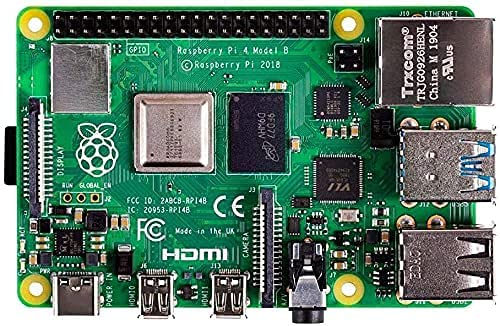
\includegraphics[scale=0.2]{rasp.jpg}
            \caption{Raspberry Pi 4}
        \end{figure}

        \subsection{Ecran LCD (Raspberry Pi) tailles}
        Avec le \textit{Raspberry Pi} un écran LCD de 7 pouces permettant d'interagir avec l'ordinateur grâce à son écran tactile. 
        \begin{figure}[h]
            \centering
            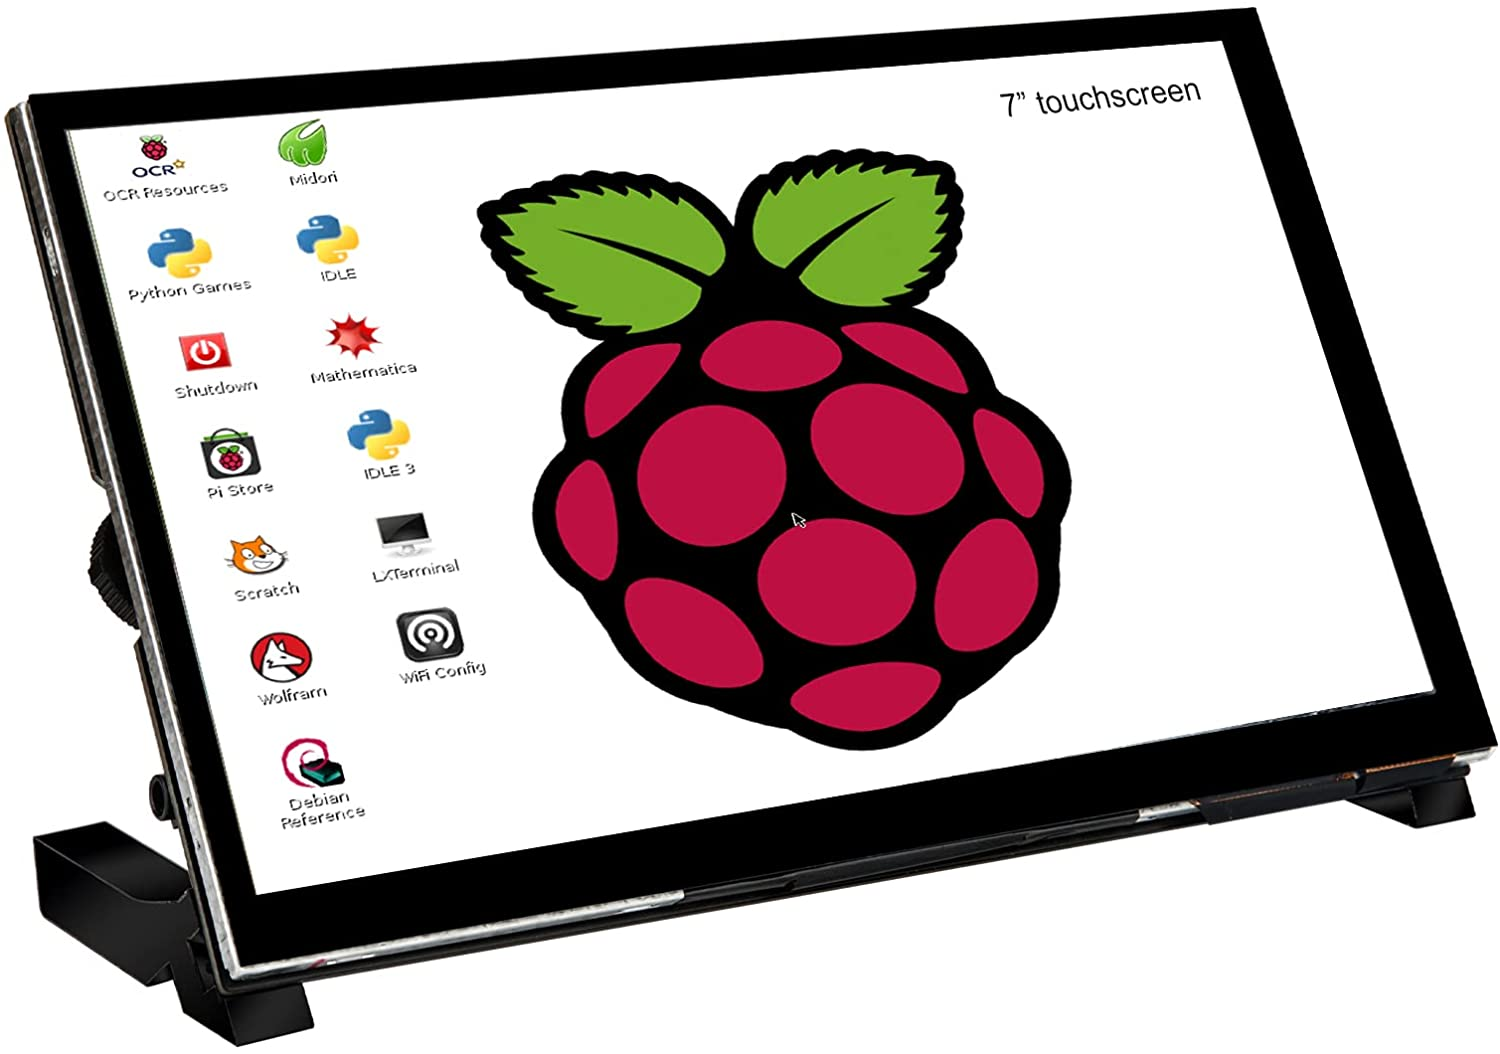
\includegraphics[scale=0.05]{ecran7p.jpg} 
            \caption{Ecran LCD de 7 pouces}
        \end{figure}

        \vspace{1cm}

        \subsection{Module de capture vidéo (Raspberry Pi) V2}
        Le module de capture vidéo (Raspberry Pi) V2 est un module de captation vidéo qui permet de capturer des images et des vidéos.
        \begin{figure}[h]
            \centering        
            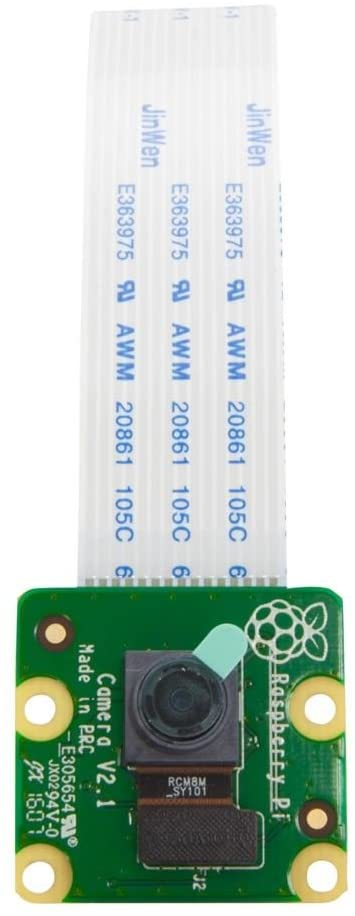
\includegraphics[scale=0.1]{module_cam.jpg}
            \caption{Module de capture vidéo (Raspberry Pi) V2}
        \end{figure}
        
    \section{Montage et Installation}
        \subsection{Installation du matériel}
        